\documentclass[12pt,a4paper]{article}
\usepackage[titletoc,toc,title]{appendix}
\usepackage{color, colortbl}
\definecolor{Gray}{gray}{0.8}
\definecolor{LightRed}{rgb}{0.99,0.9,0.9}
\usepackage{graphicx}
\usepackage{algpseudocode}
\usepackage{graphicx}
\usepackage{url}
\usepackage{verbatim}
%\usepackage{caption}
%\usepackage{subcaption}
%\usepackage{textcomp}
%\usepackage{fancyvrb}
\usepackage{graphicx}
\usepackage{amssymb}
\usepackage{epstopdf}
\usepackage[square]{natbib}
\usepackage[nottoc,numbib]{tocbibind}
\usepackage[
      pass
]{geometry}

\newcommand\todo[1]{\textcolor{red}{#1}}

\begin{document}
\title{\small Thesis\\\huge Investigating Methods Of Annotating Lifelogs For Use In Search}

\author{Harry Scells\\harrisen.scells@connect.qut.edu.au\\\\\small Supervisor - Guido Zuccon\\\small g.zuccon@qut.edu.au\\}
\maketitle
\pagebreak
\tableofcontents
\pagebreak

\section{Abstract}

\section{Introduction}

What if you had hundreds of thousands of images collected passively throughout the day and you wanted to search for events in this collection? This is a brand new, novel area of research within the domain of information retrieval \todo{[citation needed]}. A range of consumer products allow anyone to capture their daily activities and it is becoming increasingly popular \todo{[citation needed]}. The devices are typically sold under the umbrella term of "lifelogging cameras". Like blogging and vlogging before it, lifelogging is the next step in this series of life event recording devices. Not only is this an area of research for consumer products, but also has applications for security and policing services where there is a need to search the cameras which are already being worn by members of these fields.

Preliminary research has provided an insight into how difficult searching lifelogging images is. Typical search methodologies are not applicable and, until recently, there have been no freely available collections. Currently, there are no machine learning approaches which can consistently and reliably discover concepts and objects from images. Since the best option is still to annotate images manually using humans, this is what this research aims to assist with. By investigating a number of annotation methodologies and discovering which one most well suits lifelog images, we hope to provide an answer for the best way of annotating a collection of lifelog images. It is hoped that these annotations can be contributed to the wider research community to further the researach into the field of lifelog search. Supplementary data such as location, time, activity and personal health (heart rate, blood pressure, etc.) are important in pinpointing moments in time, however this research will focus on what types of annotations work best for textual search. Without meaningful annotations the supplementary information becomes useless when performing typical text-based search.

Collecting annotations is important, but determining which methodology is the best is a larger challenge. Typical textual evaluation strategies rely on a gold standard annotation. The problem becomes clear - these standard ways of evaluation are not applicable to lifelog annotations. There are currently no ways of evaluating arbitrary types of annotations for lifelog image. Designing a system for evaluating lifelog images and their annotations, and not only the types of annotations being researched by this project, but any type of annotation, will also be an important and meaningful contribution to the research community. 

\subsection{Aims and Objectives}

Four annotation methodologies have been chosen as a basis for this research. Each methodology will involve the collection of annotations through some interface and evaluation. The aim of the project is to determine, through evaluation, the best methodology for annotating lifelog images. The four methodologies under investigation are: 

\begin{enumerate}
    \item Tags --- Sets of keywords that describe objects and semantics of an image. Tags are chosen from a user-defined, non persistent vocabulary.
    \item Textual Descriptions --- Descriptive long-form annotations that contain semantic meaning.
    \item Relevance Assessments --- Images are scored on a 0-10 scale by how relevant the image relates to a given concept.
    \item Reverse Queries --- Queries are formulated for a given search result listing. Annotators are asked to provide a query that they think would result in the image being returned by a typical search engine.
\end{enumerate}

In order to collect annotations, an interface will need to be designed and developed. This will involve a website that will facilitate the collection of these annotations. Once a suitable number of annotations have been collected, each methodology will be evaluated. This will involve a novel technique, whereby the evaluation of annotations is embedded within a search task (similar to topic modelling). The evaluation will be generic, in that \textit{any} type of annotation can be submitted for evaluation. It is hoped that the methodology can be applied or built upon for future work in the area of searching lifelog images.

This research also aims to produce two meaningful contributions to the lifelog research community. Recent results from the NTCIR-12 conference indicate lifelog search engines which incorporate image processing in some way perform much better than simply using annotations alone. A new collection of \textit{well} annotated images as well as training data for image classification systems would hopefully boost the performance for everyone researching lifelog search engines. Secondly, anyone hoping to produce more annotations for a collection of lifelog images may wish to know how effective their annotation methodology is and how well it performs with respect to others. An easy to use tool for evaluation of lifelog image annotations is a necessity for this new area of research.

\subsection{Research Gaps}

The literature reviewed has revealed two gaps in the research. Annotation of lifelog images and the evaluation of them is not a standard process. Through preliminary research, a number of techniques have been investigated which are applicable to annotating images. A number of textual summarisation evaluation methods have also been discovered, however none of these are capable of evaluation without a ground truth or gold standard. Through researching the following two questions, it is hoped that these gaps in the research can be closed. According to an examination of evaluation in information retrieval systems~\citep[p. 24]{sanderson2010test}, there has been very little work done to evaluate how good a test collection is. Furthermore, finding all relevant documents to build topics is still the accepted approach for creating a test collection~\citep{cooper1973selecting}.

\subsection{Research Questions}

Two research questions have been identified by looking at previous research efforts in the literature. 

\textbf{Research Question 1:} How can annotations for a collection of lifelog images be evaluated? It is important that the annotations of images are accurate and of a high quality. Low quality annotations will lead to bad evaluation results. Evaluation will be performed without using a gold standard annotation, since this does not exist. In this way, this research will investigate a novel way of evaluating annotations for lifelog images. The most promising way to do this is through extrinsic evaluation, whereby annotations are evaluated by determining the performance of a larger system as a whole with respect to each annotation methodology. In order to keep evaluation fair, a number of baseline retrieval models will be tested to weigh out the differences between them.

\textbf{Research Question 2:} What are the possible ways lifelog images can be annotated? There are many state of the art solutions for automatically summarising the contents of images, however this project will involve manual annotations. This is due to the fact that there does not exist any training data specifically for lifelog images. This makes it challenging to train a model that can identify what is in a lifelog image. It is thought that by manually annotating images, a well formed collection of annotated lifelog images can be produced, as well as data which machine learning and computer vision algorithms can exploit.

\section{Findings From NTCIR}

The NTCIR-12 lifelogging latent semantic access task had four participants contribute to the automatic retrieval component and one participant for the interactive retrieval component. The best performing automatic team, LIG-MRIM, used computer vision to classify images and not rely on the visual concepts distributed with the task. The interactive team (LEMoRe) outperformed all other automatic teams, but this was expected as this is generally the case with tasks that have both automatic and interactive components. The other three automatic teams were VTIR, III\&CYUT and QUT (the preliminary work done for this research).

LIG-MRIM used dynamic convolutional neural networks and a multi-class support vector machine (MSVM) in order to classify images. Visual indexing is composed of two parts: three deep convolutional neural network models (AlexNet, GoogleNet and Visual Geometry Grouping (VGG)) process each image. The output is normalised and has principal component analysis (PCA) performed on it. These outputs are then concatenated together. The same normalisation and PCA process is repeated and fed into the MSVM. The output of this is concatenated with the VGG data. The second part involves temporally naming times of the day in order to attempt to extract semanitic meaning from times of the day. While this team submitted runs that fit the definition of automatic for the task, queries were generated manually from the topics by some expert.

III\&CYUT used a traditional textual based approach to lifelog retrieval. A word2vec model for the CAFFE concepts for each image was used to try to add more semantic meaning to each image. Query expansion was also used on every keyword.

The VTIR team attempted to exploit location metadata in the images. This team choose 3000 images randomly and labelled them with a rich semantic location ontology. More concepts were added by applying the WordNet database to find cognitive synonyms.

Finally, the LEMoRe team, which used an interactive approach, combined existing technologies and methodologies in order to develop a search engine. Colour correlogram, edge histogram, joint composite descriptor and pyramid histogram of oriented graphics are used by the image retrieval system as features to retrieve images. Both a novice and an expert used the system to produce runs.
\section{Literature Review}

\textbf{lit review goes here}

\section{Methods}

\subsection{Sampling Images}

The collection of lifelog images distributed for the NTCIR-12 conference far exceeds the possibility of annotating every image. The collection is very large, containing around 90,000 images. It is certainly unfeasible to annotate every image four times (for each annotation methodology), so sampling is a necessity. Previous work~\citep{scells2016qut} identified a way of clustering lifelog images based on temporal information and image histograms. After clustering images, a rough sampling technique can be performed which involves selecting one image at random from each cluster. Given more time, it would be worthwhile investigating other image similarity measures (such as those used by the LEMoRe team at NTCIR-12~\citep{de40lemore}) to possibly produce a more uniformly distributed sample set.

This sampling process reduces the total number of images needed to annotate to around 16,000. This is slightly more feasible and, intuitively, should be enough to perform some analysis on. The sampled images are uploaded into a database, ready to be annotated. This subset represents the number of annotations which will be distributed as a test collection, and the images in that test collection which have been annotated. For future work, a combination of clustering and matching images to relevant topics might be a better option, as there will most likely be many irrelevant annotations. There may also be no annotations which are relevant to a topic as well, since the sampling is somewhat random. This makes the process less than idea, but will serve as a proof of concept for further research.

\subsection{Collecting Annotations}

A test collection of accurate lifelog annotations to go along with the images is crucial for developing an effective information retrieval system or classification system. The outcomes of this thesis will be the collection of all annotations, as well as the annotation methodology or combination of methodologies which are found to be the most effective for search. This is important since annotations are only evaluated on their effectiveness for searching lifelog images, as opposed to the best annotation methodology for classifying images. This is why all of the collected annotations are made available, since the use cases for them are not limited to just typical search.

\subsubsection{Architecture}
A set of web application interfaces are used for the collection of annotations. Each interface will provide a means for an annotator to assign the respective annotation type to an image from the list of unannotated images. The architecture of these interfaces consists of:
\begin{enumerate}
    \item A database to store the annotations and the collection of images. The database will also store information about each user performing the annotations and who annotated which image. This ensures there is a record of who annotated each image, and allows for some type of analysis to be performed at a later stage.
    \item A web server that handles the "business logic". This web server exposes some password protected RESTful services that applications can hook into.
    \item Some web pages which consume the API provided by the web server and present view logic. This is the layer that annotators will interact with directly. Each interface will be one of these views.
\end{enumerate}

Annotations are inserted into the database, which can then be exported and used further down the line for other purposes such as  classifier training and evaluation. 

\subsubsection{Annotation Methodologies}

There are four annotation types under investigation. Each one is very different to the last and some interesting comparisons will hopefully be able to be drawn. There have been no studies into the most effective methodology or set of methodologies for annotating lifelog images. It would be nice to investigate more than four, however due to time constraints this is inconceivable. The annotation methodologies in question are: \textbf{textual}, \textbf{tags}, \textbf{relevance assessment} and \textbf{reverse query}. 

Each type of annotation is collected in a very similar way. An expert annotator is shown an image from the sampled collection and is asked to provide an annotation (or in the case of relevance assessment, multiple annotations) for the image. The interfaces used for collecting annotations are pictured and described as follows:

\newpage
\textbf{Textual}

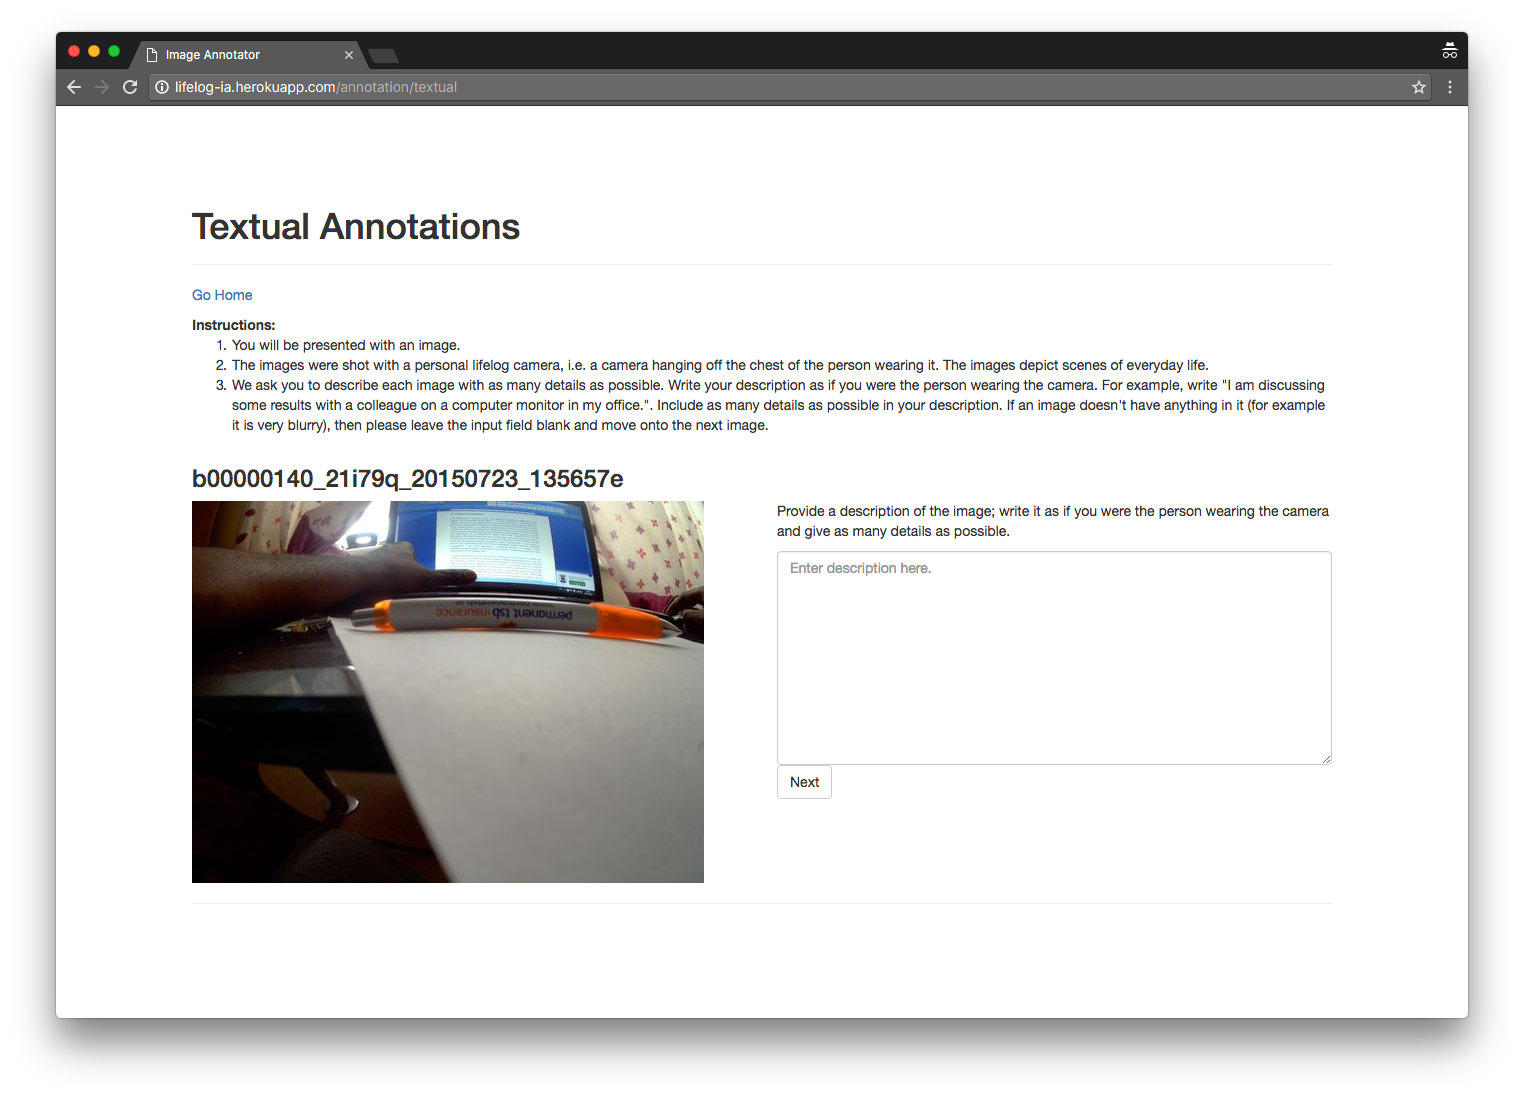
\includegraphics[width=\textwidth]{images/text-interface}

Here, annotations are collected using a text box. Free form text can be entered by the expert annotator. Textual queries should contain semantic information about an image, and should describe the image with as much detail as possible. These annotations are very similar to a textual document in a typical web search engine, which is why they were selected as one of the methodologies to investigate. These annotations may not be the best for training an image classifier, but it is hypothesised that they will perform the best in a search task.

\newpage
\textbf{Tags}

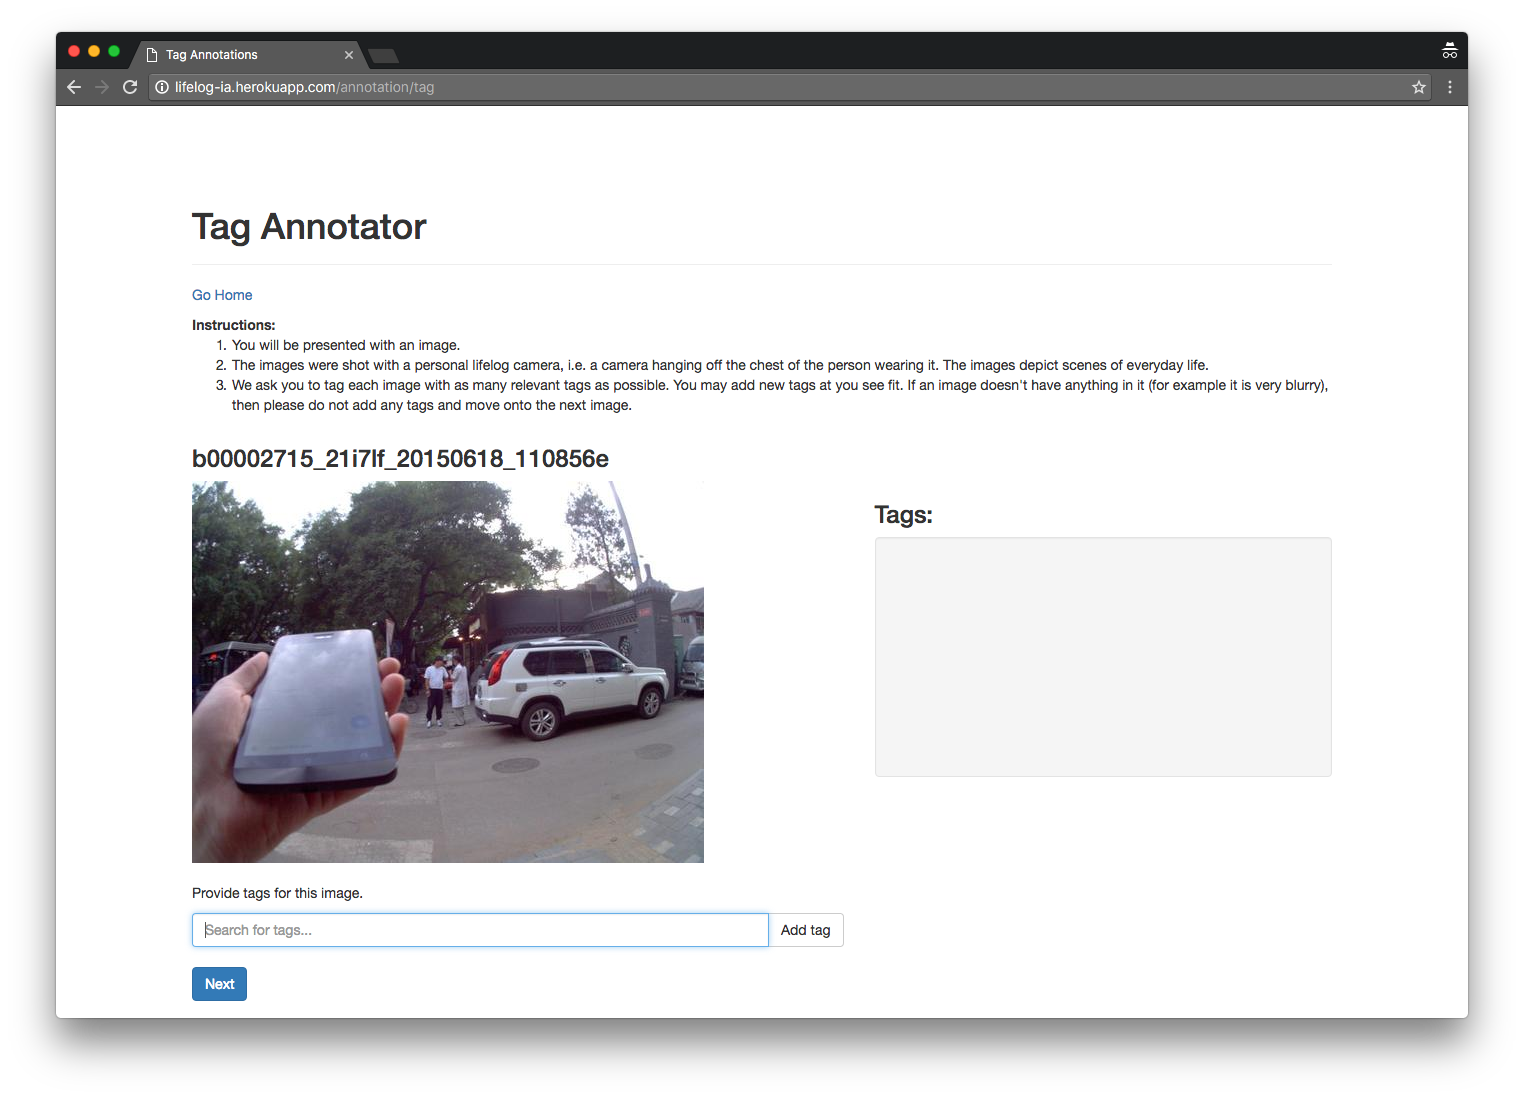
\includegraphics[width=\textwidth]{images/tag-interface}

Tags are collected through a specifically designed interface. These vocabulary of tags is created from previously added tags, meaning the list of tags available is arbitrary and can be expanded. In terms of evaluation, tags may be the opposite of textual annotations; intuitively tags should be the best at training an image classifier and are expected to perform the worst when embedded a search task. Tags, however, may be very good at boosting the performance of other annotation types in the search task when combined. For instance, searching on the text \textit{and} tags fields may increase the scores of text annotation alone.

\newpage
\textbf{Reverse Query}

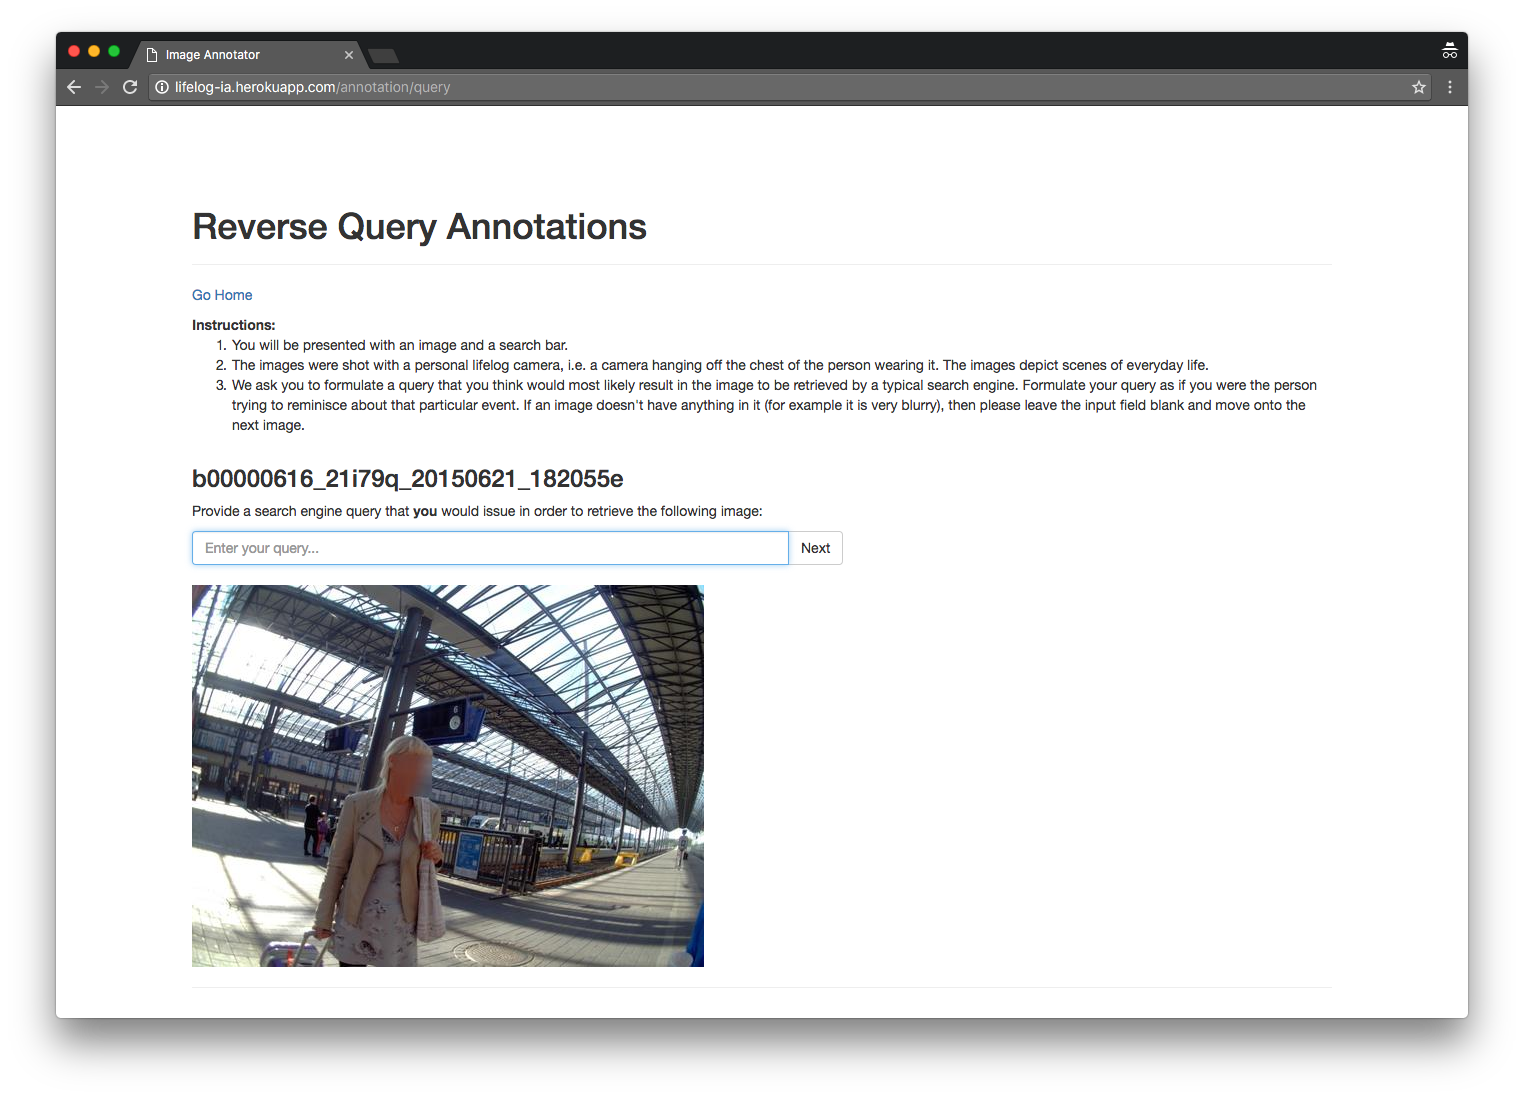
\includegraphics[width=\textwidth]{images/query-interface}

In this interface, user queries are collected by presenting an image taken from the lifelog camera and asking the annotator to provide a query with what they expect to be returned by a typical search engine. This is a relatively new and novel way to annotating \textit{any} type of document or image \todo{citation needed} and therefore it is unknown how well the collected queries will perform in search or for training an image classifier. The level of detail in these annotations will be very low, since most queries are very short \todo{citation needed}; therefore when training an image classifier, it is expected that queries will not do very well.

\newpage
\textbf{Relevance Assessment}

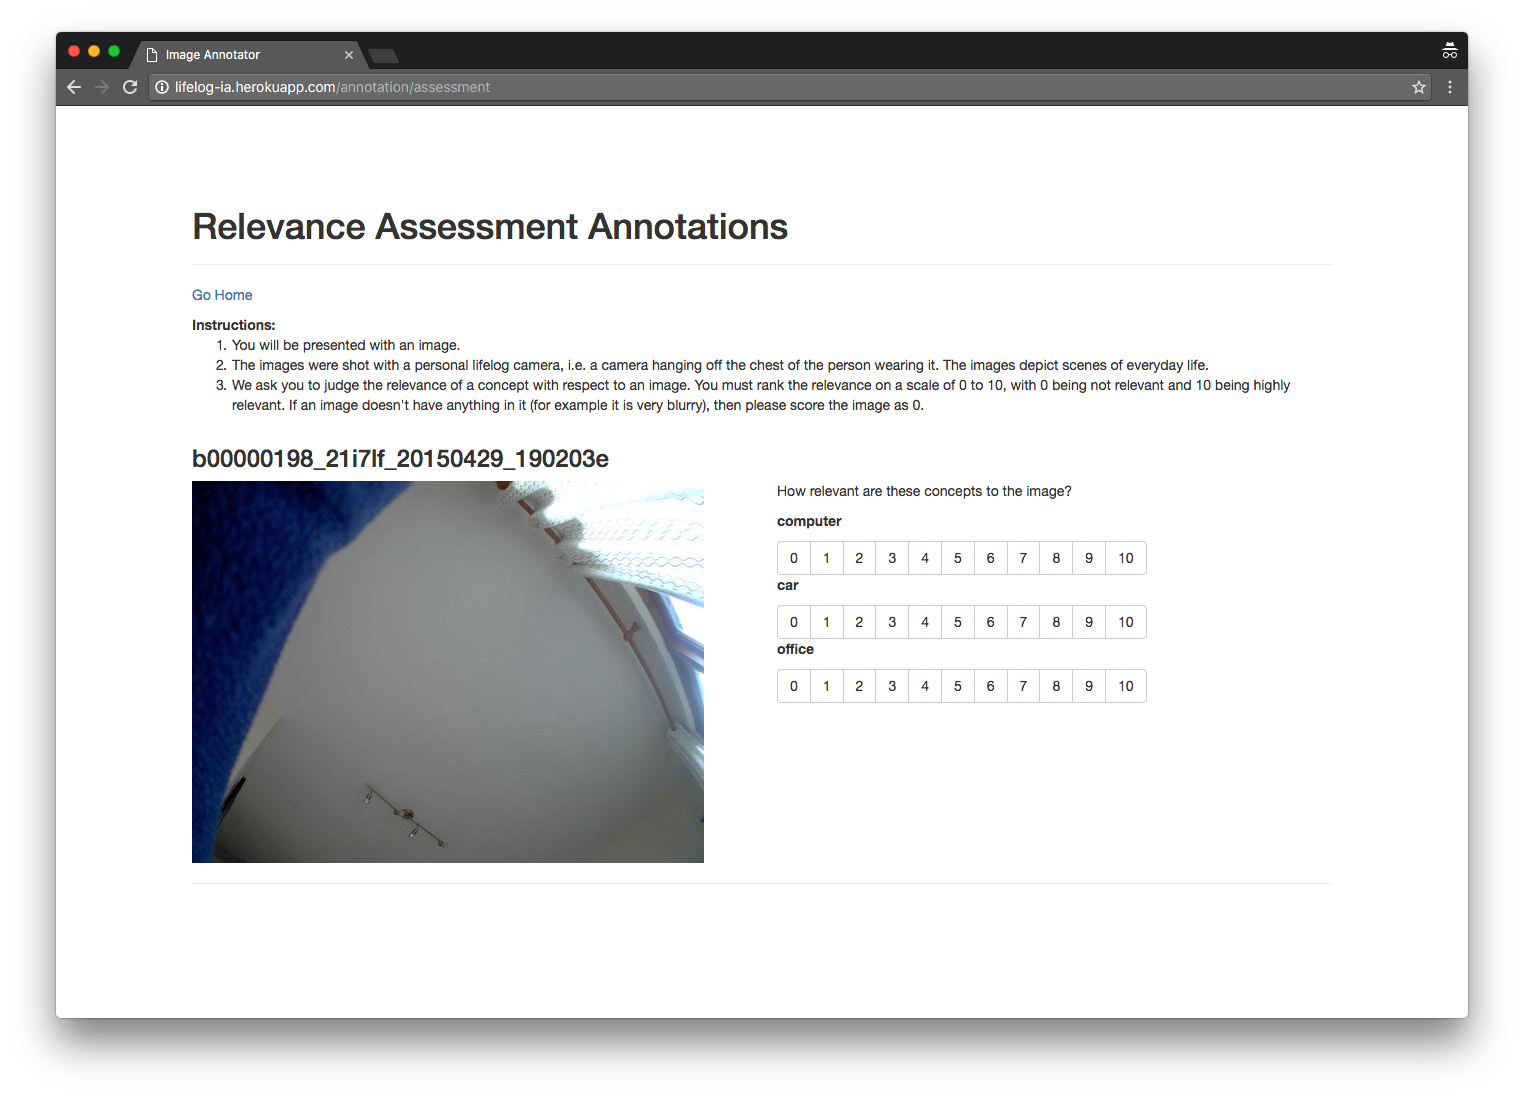
\includegraphics[width=\textwidth]{images/rel-ass-interface}

Relevance assessment involves presenting an annotator with an image, and asking them to judge how relevant a concept is to the image. These annotations will be collected last, since the list of concepts does not exist yet. It was originally planned that the concepts would be formed using a process that involved the topics from the NTCIR-12 data set. This, however, is not ideal, since the clustering process mentioned above may filter out all of the images which are relevant to a topic. It is for this reason that this annotation type will be collected last. The concepts will be formed from a combination of the previous annotations.\todo{expand on why}

\subsection{Evaluation}

\subsubsection{Evaluating Annotations}

Annotations are evaluated through statistical analysis. This will determine which annotation or combination of annotations are most effective for searching lifelog images. There is little research in evaluating test collections, however the work here will build upon previous work done by \todo{citation needed}.

A set of runs will be produced in an ad-hoc, TREC style evaluation. Every combination of annotation will be an independent run. We would like to test the combinations of annotations because, for example, the combination of tags and queries might produce better results than simply the tags or query annotations alone.

Evaluation is performed through a custom-built framework. A Java RESTful application wraps an Elasticsearch instance and performs evaluation through this. Runs are produced by issuing bulk queries to the application. The result is a set of query relevance sets (qrels) that can be evaluated through the use of trec\_eval.

\begin{enumerate}
    \item Elasticsearch is used as the information retrieval system
    \item A RESTful Java application exposes an API to add and retrieve annotations to an Elasticsearch index, as well as to perform TREC runs
    \item trec\_eval is used to evaluate the runs produced by the previous system
    \item Items two and three are repeated for every combination of annotation types using a script
\end{enumerate}

This will quantify which annotations out of the four tested are the most effective for searching lifelog images. What is arguably more important is evaluating how good the best annotations are as a test collection for lifelog images. A test collection which does not suit the needs of the topics which are being tested is not very helpful. In doing this, it will determine if the annotations are a good fit for testing a search engine system as a whole.

\subsubsection{Evaluating The Test Collection}

It may not just be good enough to evaluate how good the annotations are, it is also worthwhile to evaluate the test collection of annotations as a whole.

\section{Results}

\section{Discussion}

\section{Conclusions}

\begin{appendices}
\renewcommand\thetable{\thesection\arabic{table}}
\renewcommand\thefigure{\thesection\arabic{figure}}
\section{Format of Collection} \label{app:format}

\end{appendices}

\bibliographystyle{abbrv}
\bibliography{thesis}

\end{document}
